\documentclass{article}

% Official NeurIPS 2026 style, workshop track, camera-ready.
\usepackage[dblblindworkshop, final]{neurips_2026}
\workshoptitle{Collaborative, Open, and DECentralized training of Foundation Models}

\usepackage[utf8]{inputenc}
\usepackage[T1]{fontenc}
\usepackage{hyperref}\hypersetup{hidelinks}
\usepackage{url}
\usepackage{booktabs}
\usepackage{amsfonts}
\usepackage{amsmath}
\usepackage{wrapfig}
\usepackage{amsthm}
\usepackage{nicefrac}
\usepackage{microtype}
\usepackage{graphicx}
\usepackage{xcolor}
\usepackage{mdframed}
\usepackage{pgfplots}\pgfplotsset{compat=1.18}\usepgfplotslibrary{groupplots}

\theoremstyle{plain}
\newtheorem{theorem}{Theorem}
\newtheorem{proposition}[theorem]{Proposition}
\newtheorem{corollary}[theorem]{Corollary}

% , , , , , , , , , , , , , 

\newcommand{\sg}{\sigma_g}
\newcommand{\pg}{\varphi_{\mathrm{g}}}
\newcommand{\ps}{\varphi_{\mathrm{s}}}
\newcommand{\R}{\mathbb{R}}
\newcommand{\E}{\mathbb{E}}

\newmdenv[linewidth=0.8pt,linecolor=black!55,backgroundcolor=black!3,
          skipabove=8pt,skipbelow=8pt,innertopmargin=6pt,
          innerbottommargin=6pt]{keybox}

\title{Which Half of Participation Does the Sparse-Averaging Contraction Need?}

\author{%
  Nirodya Pussadeniya \\
  School of Information Technology, Deakin University, Australia \\
  \texttt{s226057035@deakin.edu.au}
}

\begin{document}

\maketitle

\begin{abstract}
Decentralized training synchronizes model replicas by periodically averaging a
random subset of their weights. Existing guarantees assume every replica both
contributes to the average and receives the result, although these are separate
communication events that fail independently in real systems. We audit this
assumption and find an asymmetry: send failures do not affect the leading-order
contraction of disagreement, and replicas agree exactly when every replica
receives, however few contribute; receive failures reduce the contraction
linearly. Send failures instead displace the value replicas agree on, a second
channel that doubly stochastic mixing cannot represent because it preserves the
mean by construction. The separation gives an effective averaging rate set by
the receive fraction, showing the admissible step size is smaller than
previously stated, and reveals staleness correction as a finite-time transfer of
error between the two channels. All expressions are exact for arbitrary replica
weights and validated against a faithful implementation without fitted
parameters.
\end{abstract}\vspace{-8pt}

\vspace{-17pt}\section{One Assumption, Two Events}\label{sec:audit}\vspace{-9pt}

\textbf{Setting.}\quad $m$ replicas hold weights $w_i$ and take local optimizer
steps. Periodically a random $p$-fraction of coordinates is selected, and for
each the replicas exchange values and adopt the mean. With disagreement
$\|\Delta\|^2=\sum_i\|w_i-\bar w\|^2$, the standard guarantee is that one round
contracts it to $(1-p)\|\Delta\|^2$
\citep{beton2025sparta,ajanthan2026asyncmesh}.

\textbf{Where the assumption hides.}\quad That proof sets
$w_{i:\mu} \leftarrow \frac{1}{m}\sum_j w_{j:\mu}$ for every selected coordinate
$\mu$. The left-hand side carries the replica index $i$; the right-hand side does
not. Every replica is assumed both to \textbf{contribute} to the mean and to
\textbf{adopt} it. In deployment these are two network events with independent
failure modes, instrumented separately: a permissionless 8.6B-parameter run logs
``reduce success'' and ``averaging success'' as distinct counters
\citep{avraham2026agora}. No analysis in the sparse-averaging line separates
them; the closest treatment is federated learning over noisy channels, which
finds downlink noise more damaging than uplink
\citep{wei2021noisy,upadhyay2023snr}, the analogue for channel noise of what we
prove here for participation.

\textbf{The audit.}\quad Let $\pg$ be the fraction of replicas whose values reach
the aggregator, and $\ps$ the fraction that receive the result back, drawn
independently; $\pg = \ps = 1$ recovers the standard operator. We compute one round
exactly for an \textbf{arbitrary fixed} weight configuration, with a constant
independent of it (Appendix~\ref{app:theory}): no distributional assumption and
no replica homogeneity, where the derivation it extends assumes identical
initialisation, i.i.d.\ splits and identical hyperparameters
\citep{ajanthan2026asyncmesh}. Ours therefore covers heterogeneous data, but is
one round, not a convergence guarantee under heterogeneous objectives. Per
averaged coordinate, disagreement retained is $(1-\ps) + O(1/m)$, so $\pg$ is
absent at leading order. The corresponding shift in the mean is
$\big[\ps^2(1-\pg)/\pg + \ps(1-\ps)\big]$ disagreement$/(m-1)$, where $\pg$
appears explicitly and the displacement diverges as $\pg \to 0$.

\textbf{Why existing analyses cannot express this.}\quad The standard framework
models a round as multiplication by a mixing matrix $W$ and bounds disagreement
through its spectral gap \citep{koloskova2020unified}; recent systems work models
failure as \emph{weaker mixing} under a $W$ taken ``symmetric and doubly
stochastic'' \citep{hewa2026factored}. Double stochasticity is exactly
$\mathbf{1}^\top W=\mathbf{1}^\top$, so the round preserves the mean: the send
channel is not merely unstudied there, it is zero by assumption, and no
contraction factor can express it. Our operator loses double stochasticity as
soon as the two sets differ, since columns of non-contributing replicas sum below
one. The remedy for such mixing is push-sum
\citep{kempe2003gossip,nedic2016pushsum,assran2019sgp}, which appears in no
sparse-averaging system in this line. Non-mean-preserving consensus is itself
classical \citep{fagnani2008randomized}; what is new is its composition with
sparse coordinate masking and local steps, the exact constants of both channels,
and the consequence for the step size (Appendix~\ref{app:related}). The
boundary is sharp: when the two sets coincide ($G=R$) the operator \emph{is}
doubly stochastic, retained disagreement is $m(1-\phi)/(m-1)$ and displacement is
exactly zero, below $10^{-32}$ (Appendix~\ref{app:correlated}). Correlated
failure is covered by existing theory, independent failure is not, and
deployments lie between.

The contraction therefore needs only the receive half. Send failures are close to
free for agreement and instead charge into a second channel that displaces the
value agreed upon, shrinking as $1/m$. The $\ps{=}1$ corner alone gives none of
this: not the rate for $\ps<1$, not the displacement variance, and not the
\emph{opposing} motion of the two channels as failures are reallocated
(Table~\ref{tab:asymmetry}).

\vspace{-18pt}\section{What the Audit Buys}\label{sec:buys}\vspace{-10pt}

\textbf{The admissible step size is smaller than stated.}\quad Composing the
contraction with a standard local-SGD recursion gives, for $L$-smooth
objectives, $\eta < p\,\ps/[c(1-p\,\ps)L]$ with an absolute constant $c$ that
also corrects the published $\eta<p/[2(1-p)L]$ (Appendix~\ref{app:floors}),
whose tightness \citet{ajanthan2026asyncmesh} leave open. At fixed $c$,
$\ps{=}1$ gives $\eta<p/[c(1-p)L]$, so receive failure alone \emph{narrows} the
range. The effective sparsity is $p\,\ps$, not $p$: a run
losing a quarter of its returns averages $3.75\%$ of coordinates rather than
$5\%$, so a step size tuned on the nominal $p$ exceeds this sufficient
condition. Both channels enter as floors rather than growth
rates, since the displacement is conditionally zero-mean and acts as additive
noise, so within this analysis it raises the floor rather than acting at first
order (Appendix~\ref{app:floors}).

\textbf{What a staleness corrector acts on.}\quad The split says what a delay
corrector is for, and yields a design consequence: correctors and receive-path
reliability act on the same channel and should be tuned jointly, not
independently. Delay leaves the contraction nearly unchanged and increases
displacement, so it acts on the second channel; the EMA corrector of
\citet{ajanthan2026asyncmesh} restores that displacement toward its delay-free
value and increases the disagreement left standing (Appendix~\ref{app:exact},
Table~\ref{tab:corrector}). For the corrector and delays tested, correction
moves error between channels rather than removing it, and is least attractive
where receive-path failure has already loaded the contraction channel.

\begin{wraptable}{r}{0.36\columnwidth}
\vspace{-22pt}
\centering\small
\caption{A fixed $25\%$ failure budget moved from the receive to the send path
($m{=}16$, 3 seeds). $\psi{=}\ps{+}O(1/m)$: effective receive fraction.
Loss follows $\psi$; the predicted displacement moves the opposite way,
$0.0125$ to $0.0222$.}
\label{tab:asymmetry}
\begin{tabular}{ccc}
\toprule
send/recv & $\psi$ & loss \\
\midrule
0.00/0.25 & 0.763 & 4.0584 \\
0.06/0.19 & 0.822 & 4.0521 \\
0.13/0.13 & 0.881 & 4.0449 \\
0.19/0.06 & 0.941 & 4.0382 \\
0.25/0.00 & 1.000 & 4.0328 \\
\bottomrule
\end{tabular}
\vspace{-24pt}
\end{wraptable}

This is not an artifact of operating near a known instability boundary: over two
orders of magnitude of delay the residue grows monotonically with $\Pi=\tau p$,
the stale writes in flight, from $0.015$ to $0.401$ as $\Pi$ goes $0.05$ to $1$,
while
uncorrected averaging annihilates disagreement exactly at every delay when
$\ps{=}1$ (Appendix~\ref{app:exact}, Table~\ref{tab:ei}). This does not
contradict the correction's asymptotic guarantee, which shows the spread
vanishes and identifies the post-write deviation as exactly it; we measure the
same quantity at finite time and show its value is set by $\Pi$, which the
asymptotic statement does not expose. Per seed the budget sweep is
monotone across all five splits, and three independent five-point orderings
agreeing by chance has probability ${\approx}5\times10^{-6}$.

\textbf{The operator behaves as derived.}\quad On real training weights across 11
configurations with both channels injected, prediction and measurement
agree to $3.2\times10^{-3}$ with no fitted constant (Appendix~\ref{app:exact},
Table~\ref{tab:operator}). A pre-registered prediction that the dominant failure
path would swap with replica count is \textbf{falsified} at every tested $m$,
including $m{=}4$ where the send channel is strongest
(Appendix~\ref{app:crossover}), so the rule carries no $m$-dependent caveat.

\textbf{The rule} (at the scale tested; Appendix~\ref{app:setup}).\quad
Spend reliability budget on making replicas \emph{receive} rather than send, carry $p\,\ps$ in guarantees rather than $p$,
and report a staleness corrector with the disagreement it buys back.

\bibliographystyle{plainnat}
\bibliography{refs}

\appendix
\newpage

\section{The operator, and the two theorems}\label{app:theory}

\textbf{Notation.} $\pg$ is the send (contribute) fraction and $\ps$ the receive
(adopt) fraction, exactly as in the main text; the appendices use the same two
symbols throughout. $\psi$, which appears below and in
Table~\ref{tab:asymmetry}, is the \emph{effective} receive fraction after the
finite-population correction,
\[
\psi \;=\; \ps - \frac{\ps(1-\ps)}{m-1}\Big[\frac{1-\pg}{\pg}-1\Big] \;=\; \ps + O(1/m),
\]
i.e.\ what replaces $\ps$ when the contraction is written over the whole model
rather than per coordinate. The symbol $\sg$ below denotes the residual sum
$\sum_{i\notin R}\delta_i$ and is unrelated to the send fraction.

% ===========================================================================

$m$ replicas hold weights $w_i \in \R^d$ and take local optimizer steps
between averaging rounds. Let $\bar w = \frac1m\sum_i w_i$ and let the
consensus error be $\|\Delta\|^2 = \sum_i\|w_i - \bar w\|^2$.

Each round a mask selects every coordinate independently with probability $p$.
Fix one selected coordinate and let $\delta_i = w_i - \bar w$ be the replica
deviations at it, so $\sum_i \delta_i = 0$; write $S = \sum_i \delta_i^2$.

\textbf{Complete operator (what theory assumes).} Every replica sets
$w_i \leftarrow \frac1m\sum_j w_j$. Disagreement at that coordinate becomes
zero, giving $\E\|\Delta'\|^2 = (1-p)\|\Delta\|^2$~\citep{ajanthan2026asyncmesh}.

\textbf{Incomplete operator (what systems run).} Let $G$ with $|G| = \pg m$ be
the set that reaches the reducer and $R$ with $|R| = \ps m$ the set that
receives the result, drawn uniformly and independently. The reducer forms
\begin{equation}
a \;=\; \frac{1}{|G|}\sum_{i\in G} w_i \;=\; \bar w + b,
\qquad b \;:=\; \frac{1}{|G|}\sum_{i\in G}\delta_i,
\end{equation}
and the write is $w_i' = a$ for $i \in R$, $w_i' = w_i$ otherwise.
Setting $\pg = \ps = 1$ recovers the complete operator.

\paragraph{Why this is general.} Everything below is exact for an
\emph{arbitrary fixed} $\delta$; only $G$ and $R$ are random. That is far
weaker than the homogeneous setup of~\citet{ajanthan2026asyncmesh}, identical
initialization, i.i.d.\ splits, identical hyperparameters, and data
heterogeneity does not touch it.

% ===========================================================================

% ===========================================================================

Both proofs use the finite-population identities for a uniform
$A \subseteq [m]$, $|A| = k$, over the fixed population $\{\delta_i\}$:
\begin{equation}\label{eq:fp}
\E\Big[\!\sum_{i\in A}\delta_i\Big] = 0,
\quad
\E\Big[\big(\!\sum_{i\in A}\delta_i\big)^2\Big] = \frac{k(m-k)}{m-1}\frac{S}{m},
\quad
\E\Big[\!\sum_{i\in A}\delta_i^2\Big] = \frac{k}{m}S .
\end{equation}

\begin{theorem}[The receive path sets the contraction]\label{thm:contraction}
With $S' = \sum_i(w_i' - \bar w')^2$ and $\bar w' = \frac1m\sum_i w_i'$,
\begin{equation}\label{eq:thm1}
\frac{\E[S']}{S} \;=\; (1-\ps)
  \;+\; \frac{\ps(1-\ps)}{m-1}\Big[\frac{1-\pg}{\pg}-1\Big].
\end{equation}
Over the whole model, $\E\|\Delta'\|^2 = (1-p\,\psi)\|\Delta\|^2$, with $\psi$
the effective receive fraction defined above.
\end{theorem}

\begin{proof}
Since $\bar w' - \bar w = (|R|b + \sg)/m$ with $\sg := \sum_{i\notin R}\delta_i$,
\[
S' \;=\; \sum_i (w_i'-\bar w)^2 - m(\bar w'-\bar w)^2
   \;=\; |R|\,b^2 + \!\!\sum_{i\notin R}\!\delta_i^2 - \frac{(|R|b+\sg)^2}{m}.
\]
Take $\E_G$ with $R,\delta$ fixed. By \eqref{eq:fp}, $\E_G[b] = 0$ and
$\E_G[b^2] = \frac{(m-|G|)S}{|G|m(m-1)}$, so
$\E_G[(|R|b+\sg)^2] = |R|^2\E_G[b^2] + \sg^2$ and
$\E_G[S'] = |R|(1-\frac{|R|}{m})\E_G[b^2] + \sum_{i\notin R}\delta_i^2 -
\frac{\sg^2}{m}$. Now take $\E_R$, again by \eqref{eq:fp}:
$\E_R[\sum_{i\notin R}\delta_i^2] = \frac{m-|R|}{m}S$ and
$\E_R[\sg^2] = \frac{(m-|R|)|R|}{m-1}\frac{S}{m}$. Substituting $|R| = \ps m$
and $|G| = \pg m$ gives $\frac{\ps(1-\ps)(1-\pg)}{\pg(m-1)}S + (1-\ps)S -
\frac{\ps(1-\ps)}{m-1}S$, which is \eqref{eq:thm1}.
\end{proof}

\begin{corollary}\label{cor:reads}
\textnormal{(i)} $\pg{=}\ps{=}1$ gives $\E[S'] = 0$: the complete operator's
factor $(1-p)$. \textnormal{(ii)} $\psi = \ps + O(1/m)$, so the send path is
absent from the consensus recursion to leading order. \textnormal{(iii)}
$\ps = 1$ gives $\E[S'] = 0$ for \emph{any} $\pg > 0$.
\end{corollary}

Reading (iii) is the surprise: at $\ps = 1$ the replicas agree \emph{exactly},
however few of them contributed. Away from that corner the statement is
leading-order in $1/m$, as in (ii). Sending is therefore not what the
contraction needs at leading order. So what does the send path cost?

\begin{theorem}[The send path moves the mean]\label{thm:mean}
With $v := S/m$,
\begin{equation}\label{eq:thm2}
\E\big[(\bar w' - \bar w)^2\big]
 = \frac{v}{m-1}\Big[\ps^2\,\frac{1-\pg}{\pg} + \ps(1-\ps)\Big].
\end{equation}
\end{theorem}

\begin{proof}
$\E[(\bar w'-\bar w)^2] = (|R|^2\E_G[b^2] + \E_R[\sg^2])/m^2$; substitute
\eqref{eq:fp}.
\end{proof}

The bracket holds the two channels side by side. The send term
$\ps^2(1-\pg)/\pg$ blows up as $\pg\to0$ and vanishes at $\pg = 1$. The
receive term $\ps(1-\ps)$ peaks at $\ps = \nicefrac12$ and vanishes at both
ends. At full participation both vanish and the mean is exactly preserved, as
it must be.

The prefactor is what makes this more than a curiosity: \textbf{mean
displacement is $O(1/m)$, contraction is $O(1)$.} The two channels shrink at
different rates as a deployment grows.

% ===========================================================================

\section{Derivation of the two floors}\label{app:floors}

We assume $f$ is $L$-smooth and bounded below by $f^\star$, stochastic
gradients are unbiased with variance at most $\sigma^2$, and the mask, gather
set and scatter set are drawn independently of the gradients. Write
$V_t = \E\|\Delta^t\|^2$ and $\Delta_f = f(\bar w^0) - f^\star$.

\paragraph{Step 1: the consensus recursion.} A local step expands the
disagreement in the standard way~\citep{yu2019linear}:
$\E\|\hat\Delta^{t+1}\|^2 \le (1+2\eta L)V_t + \eta^2C(m\sigma^2 + L^2V_t)$,
and Theorem~\ref{thm:contraction} contracts it, giving
\[
V_{t+1} \le (1-p\psi)\big[(1+2\eta L+\eta^2CL^2)V_t + \eta^2Cm\sigma^2\big].
\]
The recursion contracts when $(1-p\psi)\,(1+2\eta L+\eta^2CL^2) < 1$, i.e.\ when
$(1-p\psi)(2\eta L + C\eta^2L^2) < p\psi$. The condition quoted in the main text
of \citet{ajanthan2026asyncmesh}, and the form $\eta < p\psi/[2(1-p\psi)L]$ that
replaces $p$ by $p\psi$ in it, control the $2\eta L$ term alone and leave no
room for $C\eta^2L^2$, so neither is by itself sufficient. Since Step~3 already
assumes $\eta \le 1/(2L)$, we have $C\eta^2L^2 \le C\eta L/2$ and it suffices
that
\begin{equation}\label{eq:lr}
\eta \;<\; \frac{p\,\psi}{c\,(1-p\,\psi)\,L},
\qquad c = 2 + C/2 ,
\end{equation}
which is the same condition with $2$ replaced by the absolute constant $c$.
Only the admissible range of $\eta$ changes, by a constant factor; the floors
derived below are unaffected, since they follow from the fixed point in the
regime $\eta L \ll p\psi$. With \eqref{eq:lr} the fixed point satisfies
\begin{equation}\label{eq:vinf}
V_\infty \;\le\; \frac{(1-p\psi)\,\eta^2Cm\sigma^2}{1-(1-p\psi)(1+2\eta L+\eta^2CL^2)}
\;\asymp\; \frac{\eta^2Cm\sigma^2}{p\,\psi}
\end{equation}
whenever $\eta L \ll p\psi$, which is the regime \eqref{eq:lr} already
enforces: the denominator is $p\psi - (1-p\psi)(2\eta L + C\eta^2L^2)$, which
tends to $p\psi$ in that regime regardless of the constant $c$.

\paragraph{Step 2: the mean perturbation is conditionally zero-mean.} Write
$\bar w^{t+1} = \bar w^t - \eta\bar g^t + \xi^t$, where $\xi^t$ collects the
displacement of Theorem~\ref{thm:mean}. Per coordinate
$\xi = (|R|b+\sg)/m$, and by \eqref{eq:fp} both $\E_G[b] = 0$ and
$\E_R[\sg] = 0$, so $\E[\xi^t\mid\mathcal{F}^t] = 0$. Consequently $\xi^t$
contributes nothing to the inner-product term of the descent lemma and, being
independent of $\bar g^t$, nothing to the cross term either. It
enters only as $\frac{L}{2}\E\|\xi^t\|^2$, the mean-displacement term.

\emph{This is why, within this analysis, participation failure enters as a
floor rather than as a drift.} A biased perturbation would enter at first order
and compound; a zero-mean one enters at second order and behaves as additive
noise. This bounds the stationarity measure above by a quantity that does not
grow with $T$; it is not a proof that no choice of step size or failure process
can destabilise a run, and in particular it says nothing about step sizes
outside \eqref{eq:lr}.

\paragraph{Step 3: assemble.} The descent lemma with
$\|\frac1m\sum_i\nabla f(w_i)-\nabla f(\bar w)\|^2 \le \frac{L^2}{m}\|\Delta\|^2$
gives, for $\eta\le 1/(2L)$,
\[
\tfrac{\eta}{2}\E\|\nabla f(\bar w^t)\|^2
 \;\le\; \E f(\bar w^t) - \E f(\bar w^{t+1})
 + \tfrac{\eta L^2}{2m}V_t + \tfrac{L\eta^2\sigma^2}{2m}
 + \tfrac{L}{2}\Theta V_t .
\]
Telescoping over $T$ steps, dividing by $\eta/2$, and substituting
\eqref{eq:vinf} with $\psi = \ps + O(1/m)$ yields the two floors: the
$\frac{L^2}{m}V_\infty$ term becomes $L^2C\eta^2\sigma^2/(p\ps)$, and
$\frac{L}{\eta}\Theta V_\infty$ becomes
$\frac{LC\eta\sigma^2}{m-1}\big[\ps\frac{1-\pg}{\pg}+(1-\ps)\big]$. \qed

\section{Does the operator behave as derived?}\label{app:exact}

We drive the real sparse-averaging implementation with both failure channels
injected and compare predicted against measured one-round quantities on
training weights, across 11 configurations. There is no fitted constant: the
predictions are Theorems~\ref{thm:contraction} and~\ref{thm:mean} evaluated at
the run's own $(\pg,\ps,m,p)$.

\begin{table}[tb]
\centering
\caption{Measured one-round operator against Theorems~\ref{thm:contraction}
and~\ref{thm:mean}, driving the real implementation on a training transformer
($m{=}16$, $p{=}0.25$). No fitted parameters. Max deviation
$3.2\times10^{-3}$.}
\label{tab:operator}
\small
\begin{tabular}{cc cc cc}
\toprule
& & \multicolumn{2}{c}{disagreement retained}
  & \multicolumn{2}{c}{shift in the mean} \\
\cmidrule(lr){3-4}\cmidrule(lr){5-6}
$\pg$ (send) & $\ps$ (receive) & measured & Thm~\ref{thm:contraction}
              & measured & Thm~\ref{thm:mean} \\
\midrule
1.00 & 1.00 & 0.00000 & 0.00000 & 0.00000 & 0.00000 \\
0.75 & 1.00 & 0.00000 & 0.00000 & 0.02222 & 0.02222 \\
0.50 & 1.00 & 0.00000 & 0.00000 & 0.06665 & 0.06667 \\
\midrule
1.00 & 0.75 & 0.23539 & 0.23750 & 0.01243 & 0.01250 \\
1.00 & 0.50 & 0.48390 & 0.48333 & 0.01669 & 0.01667 \\
0.75 & 0.75 & 0.23844 & 0.24167 & 0.02593 & 0.02500 \\
0.50 & 0.50 & 0.49936 & 0.50000 & 0.03465 & 0.03333 \\
\bottomrule
\end{tabular}
\end{table}

The seven rows above are a representative subset of the 11 configurations
measured; the largest absolute deviation across all 11 is
$3.2\times10^{-3}$. Note the first block: at $\ps{=}1$ the disagreement
retained is $0.00000$ for every $\pg$ down to $0.50$, while the shift in the
mean grows monotonically, the two channels, separated, in one table.

\begin{table}[tb]
\centering
\caption{The same operator with a delay, and then with the EMA staleness
correction of~\citet{ajanthan2026asyncmesh}, at $\pg{=}1.0$, $\ps{=}0.75$,
$m{=}16$. Predictions are the $\tau{=}0$ values of
Theorems~\ref{thm:contraction}--\ref{thm:mean}; the departures are the point.}
\label{tab:corrector}
\small
\begin{tabular}{lcc}
\toprule
& consensus retained & shift in the mean \\
\midrule
predicted ($\tau = 0$) & 0.23750 & 0.01250 \\
measured, plain write & 0.23539 & 0.01243 \\
measured, delay $\tau{=}10$ & 0.27052 & 0.10237 \\
measured, delay $+$ EMA correction & 0.73117 & 0.01298 \\
\bottomrule
\end{tabular}
\end{table}

\begin{table}[h]
\centering\small
\caption{Disagreement left standing after one round, sweeping the delay at
$p{=}0.05$, $m{=}16$, $\pg{=}\ps{=}1$. $\Pi=\tau p$ counts the stale writes to a
coordinate in flight at once; two seeds per cell, agreeing to $5\times10^{-4}$.
The $\Pi{=}0.05$ row is the regime of the deployed run of
\citet{avraham2026agora}.}
\label{tab:ei}
\begin{tabular}{cccc}
\toprule
$\tau$ & $\Pi$ & uncorrected & EMA corrected \\
\midrule
 1 & 0.05 & 0.00000 & 0.01508 \\
 5 & 0.25 & 0.00000 & 0.08715 \\
10 & 0.50 & 0.00000 & 0.18929 \\
20 & 1.00 & 0.00000 & 0.40132 \\
\bottomrule
\end{tabular}
\end{table}

\section{Correctors in the two-channel framework}\label{app:corrector}

Table~\ref{tab:corrector} reports that a staleness corrector restores the
mean and triples the consensus error. The decomposition explains why, in one
line.

A delay-corrected write replaces the stale average with
$w_i' = \bar w^{t-\tau} + d_i$, where $d_i$ is the corrector's per-replica
estimate of the drift. Decompose it as $d_i = \bar d + e_i$ with
$\sum_i e_i = 0$. The written values now differ across replicas, so the
post-write deviation on a selected coordinate is $e_i$ rather than $0$, and
\begin{equation}
\frac{\E[S']}{S} \;=\; \frac{\E\|e\|^2}{S},
\qquad
\bar w' - \bar w \;=\; \big(\bar w^{t-\tau} + \bar d\big) - \bar w^t .
\end{equation}
The corrector's \emph{cross-replica spread} lands entirely in the contraction
channel, and its \emph{mean} entirely in the displacement channel. Any corrector
of this form reallocates error between the two channels; whether total error
falls depends on which term dominates the floor of
Appendix~\ref{app:floors}. Table~\ref{tab:corrector} measures that exchange: the mean is restored
to within $4\%$ of its delay-free value, and the contraction channel absorbs
the cost.

This also identifies when a corrector is a bad trade: when the contraction
channel already dominates the floor bound of Appendix~\ref{app:floors}. By
Theorem~\ref{thm:contraction} that is precisely the regime created by
receive-path failure, so correcting staleness and losing returns interact
badly, and the two should not be tuned independently.

\section{The crossover, tested and falsified}\label{app:crossover}
\begin{figure}[t]
    \centering
    % Generated from figures/f3_crossover.csv; do not edit by hand.
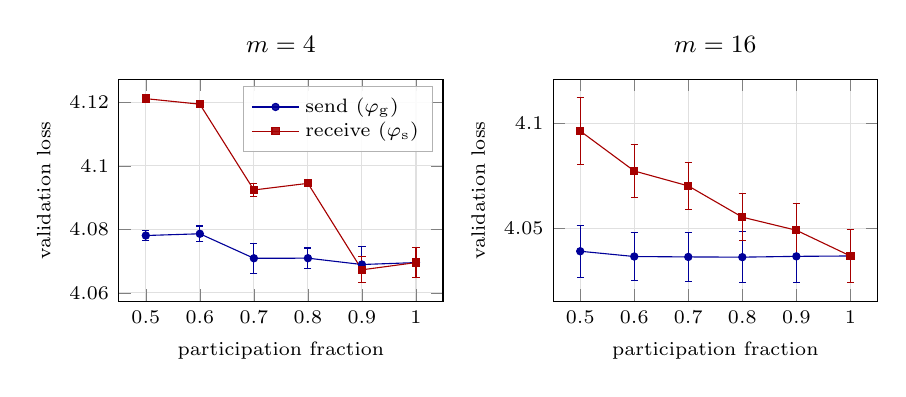
\begin{tikzpicture}
\begin{groupplot}[
  group style={group size=2 by 1, horizontal sep=1.4cm},
  width=0.47\linewidth, height=4.4cm,
  xlabel={participation fraction}, ylabel={validation loss},
  xmin=0.45, xmax=1.05, xtick={0.5,0.6,0.7,0.8,0.9,1.0},
  tick label style={font=\scriptsize}, label style={font=\scriptsize},
  title style={font=\small},
  legend style={font=\scriptsize, at={(0.97,0.97)}, anchor=north east,
                draw=black!30, fill=white, fill opacity=0.9,
                text opacity=1, row sep=-2pt},
  legend cell align=left, grid=major, grid style={black!12},
  cycle list={{blue!60!black, solid},{red!65!black, solid}},
]
\nextgroupplot[title={$m=4$}]
\addplot+[mark=*,mark size=1.3pt,error bars/.cd,y dir=both,y explicit]
  coordinates {(0.50,4.07805) +- (0,0.00152) (0.60,4.07860) +- (0,0.00244) (0.70,4.07088) +- (0,0.00468) (0.80,4.07091) +- (0,0.00321) (0.90,4.06891) +- (0,0.00558) (1.00,4.06952) +- (0,0.00477)};
\addlegendentry{send ($\varphi_{\mathrm{g}}$)}
\addplot+[mark=square*,mark size=1.3pt,error bars/.cd,y dir=both,y explicit]
  coordinates {(0.50,4.12120) +- (0,0.00026) (0.60,4.11945) +- (0,0.00118) (0.70,4.09241) +- (0,0.00216) (0.80,4.09450) +- (0,0.00020) (0.90,4.06724) +- (0,0.00408) (1.00,4.06952) +- (0,0.00477)};
\addlegendentry{receive ($\varphi_{\mathrm{s}}$)}

\nextgroupplot[title={$m=16$}]
\addplot+[mark=*,mark size=1.3pt,error bars/.cd,y dir=both,y explicit]
  coordinates {(0.50,4.03925) +- (0,0.01235) (0.60,4.03675) +- (0,0.01136) (0.70,4.03656) +- (0,0.01159) (0.80,4.03645) +- (0,0.01214) (0.90,4.03683) +- (0,0.01233) (1.00,4.03701) +- (0,0.01248)};
\addplot+[mark=square*,mark size=1.3pt,error bars/.cd,y dir=both,y explicit]
  coordinates {(0.50,4.09624) +- (0,0.01575) (0.60,4.07730) +- (0,0.01270) (0.70,4.07023) +- (0,0.01125) (0.80,4.05541) +- (0,0.01127) (0.90,4.04920) +- (0,0.01272) (1.00,4.03701) +- (0,0.01248)};
\end{groupplot}
\end{tikzpicture}

    \caption{Validation loss against participation, sweeping each path
separately at $m{=}4$ and $m{=}16$; error bars are half the seed range. The
prediction below is that the costlier curve swaps between panels. It does not:
the receive path is costlier at both replica counts.}
    \label{fig:crossover}
\end{figure}

Theorem~\ref{thm:mean}'s $1/(m{-}1)$ prefactor makes the send channel $O(1/m)$
while Theorem~\ref{thm:contraction} is $O(1)$, so there should be a replica
count below which the send path is the costlier one. It should therefore cost
more at small $m$, where the $1/(m{-}1)$ prefactor of Theorem~\ref{thm:mean} is
largest. We tested it directly and it is false over the range we can reach
(Figure~\ref{fig:crossover}).
At $m{=}4$, where the send channel is at its strongest, five times its value
at $m{=}16$, the receive path is still the costlier one, by $0.0420$ in
validation loss against a maximum seed spread of $0.0049$. At $m{=}16$ the
receive path is costlier by $0.0488$, against a seed spread of $0.0315$.

We report this as a negative result rather than removing the prediction,
because it sharpens the practical claim rather than weakening it. The send
channel is real, Theorem~\ref{thm:mean} is verified to
$3.2\times10^{-3}$ in Table~\ref{tab:operator}, but at realistic learning
rates it sits beneath the optimization noise floor even where it is largest.
The consequence is that the design rule stated in Section~\ref{sec:buys}
carries no $m$-dependent caveat.

\section{The reliability-budget sweep}\label{app:budget}

Holding the \emph{total} failure rate fixed at $25\%$ and varying only which path
absorbs it isolates the asymmetry, and shows the two channels moving in
\emph{opposite} directions, the effect no reading of the $\ps{=}1$ corner
predicts, and the end-to-end verification of Table~\ref{tab:asymmetry}. Validation loss
falls monotonically as the budget moves off the receive path onto the send path,
tracking the predicted contraction rate $\psi$ at all five splits, while the
predicted mean displacement rises along the same sweep from $0.0125$ to $0.0222$.
Per seed the all-receive minus all-send difference is $+0.0232$, $+0.0261$ and
$+0.0274$; each seed is monotone across all five splits, and three independent
five-point orderings agreeing by chance, in either direction, has
probability ${\approx}5\times10^{-6}$.

The measurements are Table~\ref{tab:asymmetry} in the main text.

\section{Perfectly correlated failure ($G=R$)}\label{app:correlated}

Failures are drawn independently in the main analysis, while real ones correlate
across the two phases. The perfectly correlated extreme is exactly solvable and
brackets the independent case.

Let the contributing and adopting sets coincide, $G=R$, with $|G|=\phi m$. The
aggregate is $a=\bar w+b$ with $b=\frac{1}{|G|}\sum_{i\in G}\delta_i$, and the
write is $w_i'=a$ for $i\in G$ and $w_i'=w_i$ otherwise. Then
\[
\bar w' - \bar w \;=\; \frac{1}{m}\Big[|G|\,b + \!\!\sum_{i\notin G}\!\delta_i\Big] \;=\; 0,
\]
since $\sum_{i\notin G}\delta_i = -\sum_{i\in G}\delta_i = -|G|b$. The mean is
preserved identically: with $G=R$ the operator is doubly stochastic and the send
channel vanishes. This is the precise sense in which the mixing framework of
\citet{koloskova2020unified} and \citet{hewa2026factored} is exactly right for
correlated failure and structurally blind to the independent case.

For the disagreement, $S'=|G|b^2+\sum_{i\notin G}\delta_i^2$; taking the
expectation over a uniform subset of size $|G|$ and using the finite-population
variance of a zero-sum population gives $\E[S']/S = m(1-\phi)/(m-1)$, which is
$(1-\phi)$ to leading order, the same rate the receive channel sets in the
independent case, as it must be since every adopting replica is also a
contributor here.

\begin{table}[h]
\centering\small
\caption{Perfectly correlated failure, $4\times10^{5}$ draws per cell. The
displacement is zero to machine precision and the retained disagreement matches
the closed form.}
\label{tab:correlated}
\begin{tabular}{ccccc}
\toprule
$m$ & $\phi$ & retained (measured) & $m(1-\phi)/(m-1)$ & displacement \\
\midrule
16 & 0.75 & 0.26638 & 0.26667 & $1.3\times10^{-33}$ \\
16 & 0.50 & 0.53392 & 0.53333 & $1.3\times10^{-33}$ \\
 4 & 0.75 & 0.33298 & 0.33333 & $3.2\times10^{-33}$ \\
 4 & 0.50 & 0.66672 & 0.66667 & $3.0\times10^{-33}$ \\
\bottomrule
\end{tabular}
\end{table}

\section{Stall and recovery}\label{app:stall}

The floor bound of Appendix~\ref{app:floors} predicts that participation failure raises a floor
rather than destabilising the recursion, so a run should stall while failures
are active and recover when they stop. We switch failures on over steps
$[2000, 4000)$ and release them, against two controls: a clean run, and two
configurations where the delay corrector is unstable at \emph{full}
participation.

The separation is complete. All three participation runs, $\ps = 0.6$,
$\ps = 0.4$, and $\pg = 0.6$, pass the divergence criterion, as does the
clean control. Both delay-corrector configurations diverge and do not recover.
Participation failure and staleness failure are therefore not two degrees of
one problem: one moves a floor, the other breaks a contraction, and in these
runs only the first recovered.

\section{Related work}\label{app:related}

Sparse parameter averaging~\citep{beton2025sparta} and its
variants~\citep{fournier2024wash} exchange random weight subsets;
\citet{lee2023partial} analyse partial averaging with pre-determined subsets in
federated learning, where a similar learning-rate/subset-size relationship
appears. \citet{ajanthan2026asyncmesh} make sparse averaging asynchronous and add
the EMA staleness correction priced here, while
\citet{douillard2023diloco} reduce communication by averaging \emph{infrequently}
rather than sparsely. \citet{maziane2026loscar} give the first guarantee
combining local steps, sparsification and overlap, and
\citet{maranjyan2026ringleader} obtain optimal time complexity under
heterogeneity, though through a server and assuming free communication. Every one
of these analyses assumes the complete, common-mask operator: all replicas
contribute, and all adopt.

That asymmetric link failure can preserve agreement while moving the value agreed
upon is classical in randomised gossip~\citep{fagnani2008randomized}, and we
claim no novelty for the phenomenon. Our contribution is to locate that
assumption inside a specific published contraction, to give the exact constants
of both channels under sparse masking with local steps, and to show what the
split implies for the admissible step size and for staleness correction.

\section{Experimental configuration}\label{app:setup}

All runs use the 45M \texttt{small} preset (6 layers, $d{=}512$, block 512,
GPT-2 tokenizer, tied embeddings) on WikiText-103, batch 8, AdamW at
$3\times10^{-4}$ with 600 warmup steps and cosine decay, weight decay 0.01,
gradient clipping 1.0, bf16 autocast. The $m$ replicas are stepped sequentially
in a single process, which makes a run bit-reproducible given its seed, a
requirement for the operator-exactness test of Appendix~\ref{app:exact}, where
predicted and measured quantities are compared on the same weights.

Sparse averaging uses the partitioned index selector of~\citet{beton2025sparta},
which splits each parameter into $\lceil 1/p \rceil$ disjoint parts and cycles
them, so the realised fraction is $1/\lceil 1/p\rceil$ rather than $p$; every
$p$ we quote is a realised fraction. Failures are injected per replica per
round, independently on the two phases: the contributing and adopting sets
are drawn as uniform subsets of exactly $\pg m$ and $\ps m$ replicas.

\paragraph{Relation to the sampling assumptions of Appendix~\ref{app:theory}.}
Two differences between the analysis and the implementation are deliberate.
First, Appendix~\ref{app:theory} places each coordinate in the mask
independently with probability $p$, whereas the partitioned selector cycles
disjoint parts. Theorems~\ref{thm:contraction} and~\ref{thm:mean} are stated
\emph{per averaged coordinate} and the operator acts on each selected coordinate
separately and identically, so the law of the mask enters only through the
realised fraction of coordinates averaged, which is the $p$ we quote; no step of
either proof uses independence across coordinates. Second, the cardinalities match. Appendix~\ref{app:theory} draws $G$ and $R$ as
uniform subsets of exactly $\pg m$ and $\ps m$ replicas, and the implementation
does the same: each round selects a uniform random subset of fixed size, not an
independent Bernoulli draw per replica. The realised cardinalities are therefore
not Binomial, and no Jensen gap in $1/\pg$ separates the prediction from the
measurement --- which is why the predicted columns of
Table~\ref{tab:operator} are the closed form evaluated at the nominal
$(\pg,\ps)$. Every run reported in this paper uses that mode; a per-coordinate
Bernoulli mode exists in the code, for modelling partial slice delivery, and is
used for no result here. At least one replica always contributes, so the
$\pg \to 0$ divergence of Theorem~\ref{thm:mean} describes rounds with few
contributors, never an empty gather set; where a coordinate's gather set would
be empty the implementation masks that coordinate out and no replica adopts
anything.

Grids, seeds and the exact argument string for every run are generated
programmatically and recorded as run manifests, and the run-level JSON summaries
are keyed by the same names, so every number here is traceable to one command.
Divergence is decided by a pre-registered rule fixed before any run (non-finite
loss; validation loss at or above $\ln V$ after step 500; or validation loss
regressing more than $0.5$ above its best), never by inspection. Code, the per-run JSON summaries behind every
table, and the camera-ready source are at
\url{https://github.com/Pusse-01/sparse-averaging-participation}.

\end{document}